\section{Limits on B-factories from $e^+ e^-$ Collisions}
For $e^+ e^-$ collisions, we make use of \madgraph again to handle our signal and background estimates.
Most of what was said about generation of events for the muon events holds here.

The total integrated luminosities at \belle is taken to be $1040.86fb^{-1}$, with \belleii to be expected to have around $100$ times this.
Since the centre of mass energy reaches $10.58\textrm{GeV}$, we can access the $\tau$ leptons here, which in our model have a very strong coupling to the scalar due to their large mass of $1.777\textrm{GeV}$.
There are two regions of interest in this scenario for the mass of the mediator: below, and above the threshold for the scalar to decay to muons.
Below this it can only decay to an $e^+ e^-$ pair, so the overall process for $m_\phi < 2m_\mu$ is

\begin{equation}
    e^+ + e^- \rightarrow \tau^+ + \tau^- + e^+ + e^-
\end{equation}

\noindent while above this threshold we decay almost exclusively to muons.

\begin{equation}
    e^+ + e^- \rightarrow \tau^+ + \tau^- + \mu^+ + \mu^-
\end{equation}

\subsection{Backgrounds}
Here we simply write down the irreducible SM background process, and let \madgraph run.
We generate $10,000$ background events for each of the two final states.
In this case, we allow the $Z$ to be a propagator, simply because it is easy to include and hard to exclude with \madgraph syntax.
However, this does not modify the result in any tangible way, as has been checked, since the energies are still well below the resonant condition for producing the $Z$.
A sample Feynman diagram is shown in Fig.\ \ref{fig:ee_tautaull_SM}.

\begin{figure}[h]
    \centering
    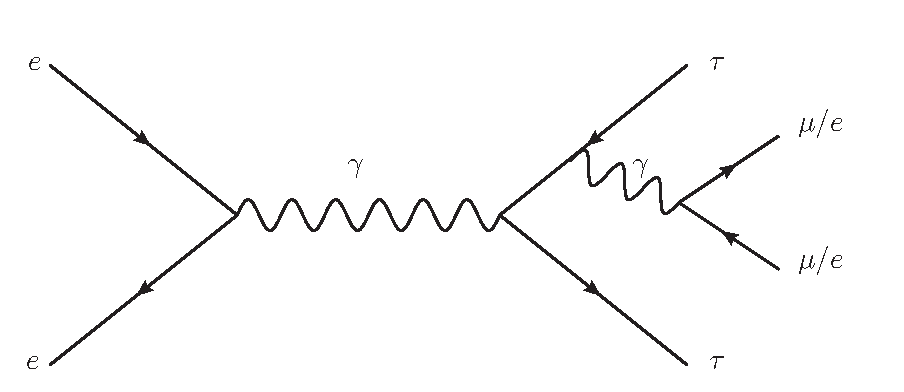
\includegraphics[width=0.6\textwidth]{Figures/feynman_diagrams/ee_tautaull_SM}
    \caption{One Feynman diagram for the background process $e^+ e^- \rightarrow \tau^+ \tau^- \ell^+ \ell^-$.}
    \label{fig:ee_tautaull_SM}
\end{figure}

\subsection{Signal}
Again, we simply define our process and let \madgraph run akin to the muon decay generation.
We enforce that the generation of the scalar is once again on-shell, so our process is really the decay chain below.

\begin{equation}
    e^+ + e^- \rightarrow \tau^+ + \tau^- + \phi,~\phi \rightarrow \ell^+ + \ell^-
\end{equation}

A sample Feynman diagram for the signal is shown in Fig.\ \ref{fig:ee_tautaull_scalar}.

\begin{figure}[h]
    \centering
    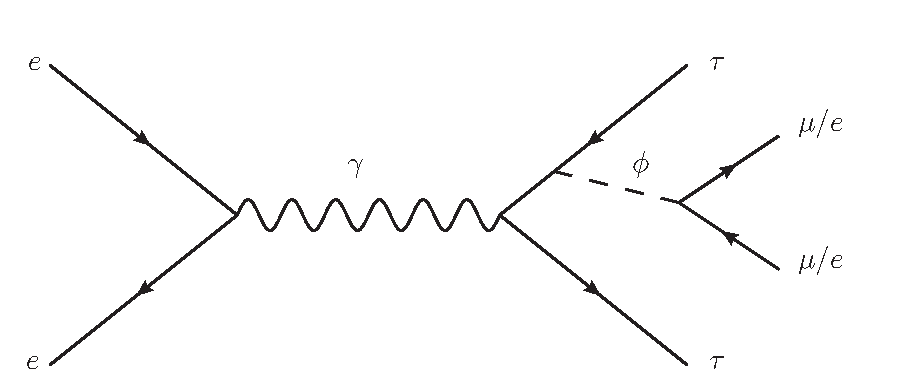
\includegraphics[width=0.6\textwidth]{Figures/feynman_diagrams/ee_tautaull_scalar}
    \caption{One Feynman diagram for the signal process $e^+ e^- \rightarrow \tau^+ \tau^- \ell^+ \ell^-$. The scalar must live on-shell before decaying promptly to a pair of leptons.}
    \label{fig:ee_tautaull_scalar}
\end{figure}
